\chapter{Opsætning af OpenCV}
\label{appendix:Opsaetning_af_opencv}

Til dette projekt bruger vi OpenCV version 2.4.9 til billedbehandling. Her gennemgås opsætningen af dette bibliotek til fremtidig reference.\newline

Opsætningen er til ingeration i linux og Qt creator. 
 
\begin{itemize}
  \item download scriptet “opencv.sh” fra dette git repository  
  \item https://github.com/jitendra29mishra/OpencvInstallation/find/master
  \item I scriptet skal version parameteren ændres til:\\  
  version="\$(wget -q -O - http://sourceforge.net/\\ projects/opencvlibrary/files/opencv-unix/2.4.9"
  item \\Scriptet er nu sat til at downloade og installere den version af OpenCV som benyttes. 
   \item Kør scriptet
   \item Start et Qt projekt og åbn .pro-filen 
   \item Åbn terminalen og tast følgende kommandoer: 
   \subitem pkg-config --cflags opencv
   \subitem pkg-config --libs opencv
   \item De ovenstående stier skal skrives i .pro-filen inden Header: og Source: eksempel ses her
     	
\begin{figure}[h] 
\centering
	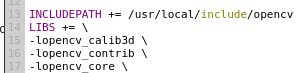
\includegraphics[width=0.5 \textwidth]{opencvQPro.PNG}
	\captionof{figure}{udklip fra Qt profil}
	\label{fig:qt_profil}
\end{figure}
  \item OpenCV headerne kan nu includes i projektets filer og funktionerne benyttes    	
    
\end{itemize}
